\documentclass{cheat-sheet}

\pdfinfo{
  /Title (Zusammenfassung Topologie)
  /Author (Tim Baumann)
}

\usepackage{tikz}
\usetikzlibrary{matrix,shapes,arrows,positioning}

\newcommand{\Tau}{\mathcal{T}} % Großes Tau
\newcommand{\inte}{\mathop{\mathrm{int}}} % Inneres (interior)
\newcommand{\conv}{\mathop{\mathrm{conv}}} % Konvexe Hülle
\newcommand{\rel}{\text{ rel }} % = relativ (Homotopie)
\newcommand{\Ob}{\mathrm{Ob}} % Objects (of a category)
\newcommand{\Hom}{\mathrm{Hom}} % Homomorphisms
\newcommand{\Aut}{\mathrm{Aut}} % Automorphisms
\newcommand{\Mor}{\mathrm{Mor}} % Morphisms
\newcommand{\dom}{\mathrm{dom}} % Domain
\newcommand{\codom}{\mathrm{codom}} % Codomain
\newcommand{\op}{\text{op}} % Duale Kategorie
\newcommand{\Deck}{\mathrm{Deck}} % Gruppe der Decktransformationen

% Kleinere Klammern
\delimiterfactor=701


\begin{document}

\maketitle{Zusammenfassung Topologie}

% Vorlesung vom 6.4.2014

\begin{defn}
  Ein \emph{metrischer Raum} $(X, d)$ besteht aus einer Menge $X$ und einer Abbildung $d : X \times X \to \R_{\geq 0}$, sodass f.a. $x,y,z \in X$ gilt:
  \begin{itemize}
    \miniitem{0.44 \linewidth}{$d(x, y) = 0 \iff x = y$}
    \miniitem{0.54 \linewidth}{$d(x, y) = d(y, x)$ \quad (Symmetrie)}
    \item $d(x, z) \leq d(x, y) + d(y, z)$ \pright{$\triangle$-Ungleichung}
  \end{itemize}
\end{defn}

% Ausgelassen: Beispiel $\R^n$
% Ausgelassen: Beispiel Funktionenraum $\mathcal{C}(\I, \R)$ mit Maximumsnorm

\begin{defn}
  Für einen metrischen Raum $(X, d)$ und eine Teilmenge $A \subset X$ ist $(A, d|_A)$ ein metrischer Raum und $d|_A$ heißt \emph{induzierte Metrik}.
\end{defn}

\begin{defn}
  Seien $(X, d_X)$ und $(Y, d_Y)$ metrische Räume. Eine Abbildung $f : X \to Y$ heißt \emph{stetig}, falls für alle $x \in X$ gilt:
  \[ \fa{\epsilon {>} 0} \ex{\delta {>} 0} \fa{x' {\in} X} d_X(x, x') < \delta \implies d_X(f(x), f(x')) < \epsilon. \]
\end{defn}

\begin{defn}
  Die \emph{offene Kugel} von Radius $\epsilon$ um $x \in X$ ist
  \[ B_\epsilon(x) \coloneqq \Set{ p \in X }{ d(p, x) < \epsilon }. \]
\end{defn}

\begin{defn}
  Eine Teilmenge $U \subset X$ eines metrischen Raumes heißt \emph{offen}, falls für alle $u \in U$ ein $\epsilon > 0$ existiert mit $B_{\epsilon}(u) \subset U$.
\end{defn}

\begin{prop}
  Eine Abbildung $f : X \to Y$ zwischen metrischen Räumen ist genau dann offen, wenn für alle offenen Teilmengen $U \subset Y$ das Urbild $f^{-1}(U) \subset X$ offen ist.
\end{prop}

\begin{defn}
  Ein \emph{topologischer Raum} $(X, \Tau)$ besteht aus einer Menge $X$ und einer Menge $\tau \subset \mathcal{P}(X)$ mit den Eigenschaften
  \begin{itemize}
    \miniitem{0.16 \linewidth}{$\emptyset \in \Tau$}
    \miniitem{0.45 \linewidth}{$\fa{U, V \in \Tau} U \cap V \in \Tau$}
    \miniitem{0.36 \linewidth}{$\fa{S \subset \Tau} \bigcap_{\mathclap{U \in S}} U \in \Tau$}
  \end{itemize}
  Die Elemente von $\Tau$ werden \emph{offene Teilmengen} von $X$ genannt. Eine Teilmenge $A \subset X$ heißt \emph{abgeschlossen}, falls $X \setminus A$ offen ist.
\end{defn}

\begin{nota}
  Seien im Folgenden $X$ und $Y$ topologische Räume.
\end{nota}

\begin{bsp}
  Die \emph{diskrete Topologie} auf einer Menge $X$ ist $\Tau = \mathcal{P}(X)$.
\end{bsp}

\begin{bsp}
  Die \emph{Klumpentopologie} auf einer Menge $X$ ist $\Tau = \{ \emptyset, X \}$.
\end{bsp}

\begin{defn}
  Die Menge der offenen Teilmengen eines metrischen Raumes heißt von der Metrik \emph{induzierte Topologie}.
\end{defn}

\begin{defn}
  Sei $(X, \Tau)$ ein topologischer Raum und $A \subset X$. Dann heißt
  \[ \Tau|_A \coloneqq \Set{U \cap A}{U \in \Tau} \]
  \emph{Unterraumtopologie} oder von $\Tau$ \emph{induzierte Topologie}.
\end{defn}

% Vorlesung vom 9.4.2014

\begin{defn}
  Ein topologischer Raum $(X, \Tau)$ heißt \emph{metrisierbar}, falls eine Metrik auf $X$ existiert, sodass die von der Metrik induzierte Topologie mit $\Tau$ übereinstimmt.
\end{defn}

\begin{defn}
  Ein topologischer Raum $(X, \Tau)$ heißt \emph{Hausdorffsch}, falls gilt:
  \[ \fa{x,y \in X} x \not= y \implies \ex{U,V \in \Tau} x \in U \wedge y \in V \wedge U \cap V = \emptyset. \]
\end{defn}

\begin{prop}
  Metrisierbare topologische Räume sind Hausdorffsch.
\end{prop}

\begin{defn}
  Eine Abbildung $f : X \to Y$ zwischen topologischen Räumen $(X, \Tau_X)$ und $(Y, \Tau_Y)$ heißt \emph{stetig}, falls gilt
  \[ \fa{U \in \Tau_Y} f^{-1}(U) \in \Tau_X. \]
\end{defn}

\begin{nota}
  $\mathcal{C}(X, Y) \coloneqq \Set{ f : X \to Y }{\text{$f$ stetig}}$
\end{nota}

\begin{bem}
  Ist $f : X \to Y$ stetig und $A \subset X$, so ist auch $f|_A : A \to Y$ stetig.
\end{bem}

\begin{defn}
  Falls $f : X \to Y$ bijektiv ist und sowohl $f$ als auch $f^{-1}$ stetig sind, so heißt $f$ ein \emph{Homöomorphismus}.
\end{defn}

\begin{defn}
  Zwei topologische Räume $X$ und $Y$ heißen \emph{homöomorph} (notiert $X \approx Y$), wenn ein Homöomorphismus zwischen $X$ und $Y$ existiert.
\end{defn}

\begin{satz}
  Für $n \not= m$ sind $\R^n$ und $\R^m$ nicht homöomorph.
\end{satz}

\begin{defn}
  Sei $X$ eine Menge und $\Tau, \Tau'$ Topologien auf $X$. Dann sagen wir
  \[ \Tau \text{ ist \emph{gröber} als } \Tau' \coloniff \Tau' \text{ ist \emph{feiner} als } \Tau \coloniff \Tau \subseteq \Tau'. \]
\end{defn}

% Bemerkung: Die Klumpentopologie ist die gröbste und die diskrete Topologie die feinste Topologie auf $X$.

\begin{defn}
  Eine Menge $\mathcal{B} \subset \Tau$ offener Teilmengen eines topologischen Raumes heißt
  \begin{itemize}
    \item \emph{Basis} der Topologie, falls jede offene Menge $U \in \Tau$ Vereinigung von Mengen aus $\mathcal{B}$ ist.
    \item \emph{Subbasis} der Topologie, falls jede offene Menge $U \in \Tau$ Vereinigung von Mengen ist, von denen jede Schnitt endlich vieler Mengen aus $\mathcal{B}$ ist.
  \end{itemize}
\end{defn}

\begin{bspe}
  \begin{itemize}
    \item Sei $(X, d)$ ein metrischer Raum. Dann ist $\mathcal{B} \coloneqq \Set{B_\epsilon(x)}{x \in X, \epsilon > 0}$ eine Basis der induz. Topologie auf $X$.
    \item $\mathcal{B} \coloneqq \Set{B_\epsilon(x)}{x \in \Q^n, \epsilon \in \Q_{+}}$ ist eine abz. Basis von $(\R^n, \d_{\text{eukl}})$.
  \end{itemize}
\end{bspe}

\begin{prop}
  Jede Teilmenge $\mathcal{B} \subset \mathcal{P}(X)$ ist Subbasis von genau einer Topologie $\Tau$ von $X$.
\end{prop}

\begin{defn}
  Die Topologie heißt die von $\mathcal{B}$ \emph{erzeugte Topologie}.
\end{defn}

\begin{defn}
  Sind $(X, \Tau_X)$ und $(Y, \Tau_Y)$ topologische Räume, so ist auch $(X \times Y, \Tau_X \otimes \Tau_Y)$ ein topologischer Raum mit der \emph{Produkttopologie} $(\Tau_X \otimes \Tau_Y)$, die von
  \[
    \mathcal{B} \coloneqq \Set{U \times Y}{U \in \Tau_X} \cup \Set{X \times V}{V \in \Tau_Y}
    \quad \text{erzeugt wird.}
  \]
  % Ausgelassen: "`Streifen"' und "`Rechtecke"'
\end{defn}

\begin{prop}
  \begin{itemize}
    \item Die Projektionen $\pi_X : X \times Y \to X$ und $\pi_Y : X \times Y \to Y$ sind stetig bzgl. der Produkttopologie.
    \item Ist $\Tau$ eine echt gröbere Topologie auf $X \times Y$ als die Produkttopologie, so sind die Projektionen $\pi_X$ und $\pi_Y$ nicht beide stetig.
  \end{itemize}
\end{prop}

% Bemerkung: Die Produkttopologie ist somit die gröbste Topologie auf $X \times Y$, sodass beide Projektionen stetig sind.

\begin{defn}
  Seien $(X, \Tau_X)$ und $(Y, \Tau_Y)$ topologische Räume. Dann erzeugt $\Tau_X \cup \Tau_Y$ die \emph{Summentopologie} auf $X \cup Y$.
\end{defn}

\begin{bem}
  Sie ist die feinste Topologie auf $X \cup Y$, sodass die beiden Inklusionen $i_X : X \hookrightarrow X \cup Y$ und $i_Y : Y \hookrightarrow X \cup Y$ stetig sind.
\end{bem}

\begin{prop}
  Seien $X, Y, Z$ topologische Räume.
  \begin{itemize}
    \item Falls $X \cap Y = \emptyset$, so ist eine Abbildung $f : X \cup Y \to Z$ genau dann stetig, falls die beiden Kompositionen $f \circ i_X : X \to Z$ und $f \circ i_Y : Y \to Z$ stetig sind.
    \item Eine Abb. $g : Z \to X \cup Y$ ist genau dann stetig, wenn die beiden Kompositionen $\pi_X \circ g : Z \to X$ und $\pi_Y \circ g : Z \to Y$ stetig sind.
  \end{itemize}
\end{prop}

\begin{defn}
  Sei $X$ ein topologischer Raum und $A \subset X$. Dann ist das \emph{Innere} von $A$ (notiert $\inte(A)$) die Vereinigung aller in $A$ enthaltenen offenen Mengen.
\end{defn}

\begin{bem}
  Als Vereinigung offener Mengen ist das Innere offen.
\end{bem}

% $\inte(A)$ ist die größte in $A$ enthaltene in $X$ offene Teilmenge.

\begin{defn}
  Der \emph{Abschluss} $\overline{A}$ einer Menge $A \subset X$ ist der Durchschnitt aller abgeschlossenen Mengen von $X$, die $A$ enthalten.
\end{defn}

\begin{bem}
  Es gilt $\overline{A} = X \setminus (\inte(X \setminus A))$.
\end{bem}

\begin{defn}
  Es sei $X$ ein topologischer Raum, $x \in X$ und $V \subset X$. Wir nennen $V$ eine \emph{Umgebung} von $x$, falls es eine offene Teilmenge $U \subset X$ gibt mit $x \in U$ und $U \subset V$.
\end{defn}

\begin{prop}
  Ein Punkt $x \in X$ liegt genau dann in $\overline{A}$, falls jede Umgebung von $x$ einen Punkt aus $A$ enthält.
\end{prop}

\begin{defn}
  Der \emph{Rand} einer Menge $A \subset X$ ist $\partial A \coloneqq \overline{A} \setminus \inte(A)$.
\end{defn}

\begin{prop}
  Ein Punkt $x \in X$ liegt genau dann in $\partial X$, wenn jede Umgebung von $x$ sowohl einen Punkt aus $A$ wie einen Punkt aus $X \setminus A$ enthält.
\end{prop}

% Vorlesung vom 14.4.2014

% Thema: Zusammenhang und Wegzusammenhang

\begin{defn}
  Ein topologischer Raum $X$ heißt \emph{wegweise zusammen- hängend}, falls es für je zwei Punkte $x, y \in X$ eine stetige Abbildung $\gamma : \I \to X$ mit $\gamma(0) = x$ und $\gamma(1) = y$ gibt.
\end{defn}

\begin{bspe}
  \begin{itemize}
    \item $\R^n$ ist wegzusammenhängend
    \item $(\{ p, q \}, \{ \emptyset, \{ p \}, \{ p, q \} \})$ ist wegzusammenhängend!
    \item $\ointerval{-\infty}{0} \cup \ointerval{0}{\infty} \subset \R$ ist nicht wegzusammenhängend.
  \end{itemize}
\end{bspe}

\begin{defn}
  Die Äquivalenzklassen von
  \[ x \sim y \coloniff x, y \text{ lassen sich durch einen Weg verbinden}. \]
  heißen \emph{Wegzusammenhangskomponenten}.
\end{defn}

\begin{prop}
  Sei $f : X \to Y$ stetig und $X$ wegzusammenhängend. Dann ist auch $f(X)$ bzgl. der Unterraumtopologie wegzusammenhängend.
\end{prop}

\begin{defn}
  Ein topologischer Raum $X$ heißt \emph{zusammenhängend}, falls $X$ nicht disjunkte Vereinigung zweier nichtleerer offener Teilmengen ist.
\end{defn}

\begin{bspe}
  $\Q \subset \R$ und $\R \setminus \{ 0 \}$ sind nicht zusammenhängend.
\end{bspe}

\begin{prop}
  Sei $X$ ein topologischer Raum. Es sind äquivalent:
  \begin{itemize}
    \item $X$ ist zusammenhängend.
    \item Für jede offene und abgeschlossene Menge $A \subset X$ gilt: $A \in \{ X, \emptyset \}$.
    \item Jede stetige Abbildung $f : X \to \{ 0, 1 \}$ in den diskreten Raum mit zwei Elementen ist konstant.
  \end{itemize}
\end{prop}

\begin{prop}
  \begin{itemize}
    \item Sei $f : X \to Y$ stetig und $X$ zusammenhängend, dann ist auch $f(X)$ zusammenhängend.
    \item Sind $A, B$ zusammenhängende Teilmengen eines topologischen Raumes $X$ und gilt $A \cap B \not= \emptyset$, dann ist auch $A \cup B$ zusammenhängend.
  \end{itemize}
\end{prop}

\begin{kor}
  Folgende Relation ist eine Äquivalenzrelation auf $X$:
  \begin{align*}
    x \sim y \coloniff \, &\text{$x$ und $y$ liegen beide in einem zusammenhängenden}\\[-2pt]
    &\text{Unterraum von $X$.}
  \end{align*}
\end{kor}

\begin{defn}
  Die Äquivalenzklassen dieser Relation heißen \emph{Komponenten}. % von $X$
\end{defn}

\begin{bsp}
  Die Komponenten von $\Q \subset \R$ sind genau die Ein-Punkt-Mengen. Trotzdem ist $\Q$ nicht diskret!
\end{bsp}

\begin{prop}
  Die Menge $\I$ ist zusammenhängend.
\end{prop}

\begin{kor}
  Wegzusammenhängende Räume sind zusammenhängend.
\end{kor}

\begin{prop}[ZWS]
  Sei $f : \I \to \R$ stetig. Gilt $f(0) < 0$ und $f(1) > 0$, so existiert ein $t \in \ointerval{0}{1}$ mit $f(t) = 0$.
\end{prop}

% Vorlesung vom 16.4.2014

\begin{defn}
  Sei $(x_n)_{n \in \N}$ eine Folge in $X$. Die Folge $(x_n)$ \emph{konvergiert gegen} $x \in X$, falls für jede Umgebung $U \subset X$ von $x$ ein $N \in \N$ existiert mit $\fa{n \geq N} x_n \in U$.
\end{defn}

\begin{nota}
  $x = \lim_{n \to \infty} x_n$
\end{nota}

\begin{acht}
  Das "`="' ist nicht wörtlich zu verstehen!
\end{acht}

\begin{defn}
  Sei $f : X {\to} Y$ eine Abb. zw. topol. Räumen $X, Y$. Dann heißt $f$
  \begin{itemize}
    \item \emph{stetig in} $x \in X$, falls für jede Umgebung $V \subset Y$ von $f(x)$ das Urbild $f^{-1}(V) \subset X$ eine Umgebung von $x$ ist.
    \item \emph{folgenstetig in} $x \in X$, falls für jede Folge $(x_n)_{n \in \N}$ in $X$ mit $\lim_{n\to\infty} x_n = x$ die Bildfolge $(f(x_n))$ in $Y$ gegen $f(x)$ konvergiert.
  \end{itemize}
\end{defn}

\begin{prop}
  Ist $f$ stetig in $x$, so ist $f$ auch folgenstetig in $x$.
\end{prop}

\begin{defn}
  Eine \emph{Umgebungsbasis} von $x \in X$ ist eine Menge $\mathcal{B} \subset \mathcal{P}(X)$ bestehend aus Umgebungen von $x$, sodass jede Umgebung von $x$ eine der Umgebungen in $\mathcal{B}$ enthält.
\end{defn}

\begin{defn}
  Der Raum $X$ erfüllt das \emph{erste Abzählbarkeitsaxiom}, falls jeder Punkt $x \in X$ eine abzählbare Umgebungsbasis besitzt.
\end{defn}

\begin{bem}
  Jeder metrische Raum $X$ erfüllt das erste Abzählbarkeitsaxiom, da für jeden Punkt $x \in X$ die Menge $\mathcal{B}_x \coloneqq \Set{B_{1/n}(x)}{n\in\N}$ eine abzählbare Umgebungsbasis ist.
\end{bem}

\begin{prop}
  Sei $x \in X$ ein Punkt mit abzählbarer Umgebungsbasis. Dann ist jede in $x$ folgenstetige Abbildung $f : X \to Y$ auch stetig in $x$.
\end{prop}

\begin{defn}
  Eine \emph{gerichtete Menge} ist eine Menge $D$ mit einer partiellen Ordnung $(\le) \subset D \times D$, sodass es für $\alpha, \beta \in D$ immer ein $\gamma \in D$ mit $\gamma \geq \alpha$ und $\gamma \geq \beta$ gibt.
\end{defn}

\begin{defn}
  Ein \emph{Netz} in $X$ ist eine Abbildung $\phi : D \to X$, wobei $D$ eine gerichtete Menge ist.
\end{defn}

\iffalse
\begin{bspe}
  \begin{itemize}
    \item $D = (\N, \leq)$
    \item $X$ beliebige Menge, $D = (\mathcal{P}(X), \subseteq)$ oder $D = (\mathcal{P}(X), \supseteq)$
    \item Sei $(X, \tau)$ ein top. Raum, $x \in X$, $D \coloneqq (\Set{U \subset X}{\text{$U$ Umgebung von $x$}}, \leq)$ mit $U \leq V \coloneqq V \subset U$.
  \end{itemize}
\end{bspe}
\fi

\begin{defn}
  Sei $x \in X$ und $(x_\alpha)_{\alpha \in D}$ ein Netz in $X$. Das Netz $(x_\alpha)$ \emph{konvergiert} gegen $x$, falls es für jede Umgebung $U \subset X$ von $x$ ein $\beta \in D$ gibt mit $x_\alpha \in U$ für alle $\alpha \geq \beta$.
\end{defn}

\begin{nota}
  $\lim_{\alpha \in D} x_\alpha = x$
\end{nota}

\begin{defn}
  Eine Abb. $f : X \to Y$ heißt \emph{netzstetig} in $x \in X$, falls für jedes Netz $(x_\alpha)_{\alpha \in D}$ in $X$ mit $\lim_{\alpha \in D} x_\alpha = x$ das Bildnetz $(f(x_\alpha))_{\alpha \in D}$ gegen $f(x)$ konvergiert.
\end{defn}

\begin{prop}
  Eine Abbildung $f : X \to Y$ ist genau dann stetig in $x \in X$, wenn sie netzstetig in $x$ ist.
\end{prop}

\begin{prop}
  Ist $A \subset X$ eine Teilmenge eines topologischen Raumes, so besteht $\overline{A}$ genau aus den Limiten von Netzen in $A$, die in $X$ konvergieren.
\end{prop}

\begin{defn}
  Ein \emph{Häufungspunkt} eines Netzes $(x_\alpha)_{\alpha \in D}$ in $X$ ist ein Punkt $x \in X$, sodass für jede Umgebung $U \subset X$ von $x$ das Netz \emph{häufig} in $U$ ist, d.\,h. für alle $\alpha \in D$ existiert ein $\beta \geq \alpha$ mit $x_\beta \in U$.
\end{defn}

\begin{defn}
  Sind $D$ und $E$ gerichtete Mengen, so nennen wir eine Abbildung $h : E \to D$ \emph{final}, falls für alle $\delta \in D$ ein $\eta \in E$ existiert mit $h(\gamma) \geq \delta$ für alle $\gamma \geq \eta$.
\end{defn}

\begin{defn}
  Ein \emph{Unternetz} eines Netzes $\phi : D \to X$ ist eine Komposition $\phi \circ h : E \to X$ wobei $h : E \to D$ eine finale Funktion ist. Wir schreiben auch $(x_{h(\gamma)})_{\gamma \in E}$
\end{defn}

% Vorlesung vom 23.4.2014

\begin{prop}
  Sei $(x_\alpha)_{\alpha \in D}$ ein Netz in $X$. Ein Punkt $x \in X$ ist genau dann Häufungspunkt von $(x_\alpha)$, falls ein Unternetz von $(x_\alpha)$ gegen $x$ konvergiert.
\end{prop}

\begin{defn}
  Eine Folge $(x_n)_{n \in \N}$ in einem metrischen Raum $(X, d)$ heißt \emph{Cauchy-Folge}, falls es für jedes $\epsilon > 0$ ein $N \in \N$ gibt mit $d(x_n, x_m) < \epsilon$ für alle $n, m \geq N$.
\end{defn}

\begin{defn}
  Der metrische Raum $(X, d)$ heißt \emph{vollständig}, wenn jede Cauchy-Folge in $X$ konvergiert.
\end{defn}

% Beispiele:
% * Wenn $(X_1, d_1)$ und $(X_2, d_2)$ vollständig, dann auch $(X_1 \times X_2, d)$ mit $d((x_1, x_2), (y_1, y_2)) \coloneqq \sqrt{d_1(x_1, y_1)^2 + d_2(x_2, y_2)^2}$
% * $\R^n$ ist vollständig
% * Ist $X$ vollständig und $A \subset X$ abgeschlossen, dann ist auch $A$ mit der induzierten Metrik vollständig
% * Ist allgemeiner $A \subset X$ ein beliebiger Unterraum, dann ist $\overline{A} \subset X$ der kleinste vollständige Unterraum, der $A$ enthält

\begin{acht}
  Vollständigkeit ist keine Homöomorphieinvariante!
  % Gegenbeispiel: $\ointerval{0}{1} \approx \R$, aber $\R$ ist vollständig, $\ointerval{0}{1}$ ist es nicht
\end{acht}

\begin{defn}
  Sei $X$ eine Menge. Dann ist die Menge
  \[ \mathcal{B}(X) \coloneqq \Set{ f : X \to \R }{ \sup_{x \in X} \abs{f(x)} < \infty } \]
  der \emph{beschränkten Fktn.} $X \to \R$ ein metrischer Raum mit
  \[ d(f, g) \coloneqq \sup_{x \in X} \abs{f(x) - g(x)}. \]
\end{defn}

\begin{prop}
  Dieser Raum $(\mathcal{B}(X), d)$ ist vollständig.
\end{prop}

\begin{defn}
  Sie $(X, d)$ und $(X', d')$ metrische Räume, so heißt $f : X \to X'$
  \begin{itemize}
    \item eine \emph{isometrische Einbettung}, falls für alle $x , y \in X$ gilt:
    \[ d'(f(x), f(y)) = d(x, y) \]
    \item eine \emph{Isometrie}, falls $f$ zusätzlich bijektiv ist. In diesem Fall ist auch $f^{-1}$ eine Isometrie und $f$ ein Homöomorphismus.
  \end{itemize}
\end{defn}

\begin{prop}
  Sei $X$ ein metrischer Raum. Dann gibt es eine isome- trische Einbettung von $X$ in einen vollständigen metrischen Raum.
\end{prop}

% Ausgelassen: Konstruktion der Kuratowski-Einbettung im Beweis.

\begin{defn}
  Eine \emph{Vervollständigung} eines metrischen Raumes $X$ ist ein vollständiger metrischer Raum $Y$ mit einer isometrischen Einbettung $f : X \to Y$, sodass $f(X)$ \emph{dicht} in $Y$ liegt, d.\,h. $\overline{f(X)} = Y$.
\end{defn}

\begin{satz}
  Für jeden metrischen Raum existiert eine Vervollständigung. % $X \hookrightarrow Y$.
\end{satz}

\begin{prop}
  Es sei $X$ ein metrischer Raum und es seien
  \[ f_1 : X \to Y_1, \quad f_2 : X \to Y_2 \]
  Vervollständigungen von $X$. Dann existiert genau eine Isometrie $\phi_{21} : Y_1 \to Y_2$ mit $\phi_{21}|_{f_1(X)} = f_2 \circ f_1^{-1}$.
\end{prop}

\begin{bsp}
  Die kanonische Inklusion $C_c^{\infty}(U) \hookrightarrow L^p(U)$ ist eine Vervollständigung von $(C_c^{\infty}, d_p)$ mit
  \[ d_p(f, g) \coloneqq \left( \Int{U}{}{\abs{f(x) - g(x)}^p}{x} \right)^{1/p}. \]
\end{bsp}

\begin{defn}
  Es sei $X$ ein topologischer Raum. Eine \emph{offene Überdeckung} von $X$ ist eine Familie $(U_i)_{i \in I}$ offener Teilmengen von $X$ mit $\bigcup_{i \in I} U_i = X$.
\end{defn}

\begin{defn}
  Der Raum $X$ heißt \emph{kompakt}, falls jede offene Überdeckung von $X$ eine endliche Teilüberdeckung besitzt, also eine endliche Teilmenge $I_0 \subset I$ mit $\bigcup_{i \in I_0} U_i = X$.
\end{defn}

\begin{defn}
  Eine Familie $\mathcal{C}$ von Teilmengen von $X$ habe die \emph{endliche Schnitteigenschaft}, falls der Schnitt je endlich vieler Mengen aus $\mathcal{C}$ nichtleer ist.
\end{defn}

\begin{prop}
  Ein Raum $X$ ist genau dann kompakt, falls jede Familie $(C_i)_{i \in I}$ von abgeschlossenen Teilmengen von $X$, die die endliche Schnitteigenschaft besitzt, einen nichtleeren Schnitt hat. %, d.\,h. $\bigcap_{i \in I} C_i \not= \emptyset$.
\end{prop}

\begin{bem}
  Kompaktheit ist eine Homöomorphieinvariante.
\end{bem}

\begin{prop}
  Jede kompakte Teilmenge eines Hausdorffraumes ist abgeschlossen.
\end{prop}

\begin{prop}
  Ist $X$ kompakt und $f : X \to Y$ stetig, so ist auch $f(X) \subset Y$ kompakt.
\end{prop}

\begin{prop}
  Jeder abgeschlossene Teilraum eines kompakten Raumes ist kompakt.
\end{prop}

\begin{prop}
  Sei $f : X \to Y$ eine bijektive stetige Abbildung von einem kompakten Raum in einen Hausdorffraum. Dann ist $f$ ein Homöomorphismus.
\end{prop}

% Vorlesung vom 30.4.2014

\begin{prop}
  Das Einheitsintervall $\I \subset \R$ ist kompakt.
\end{prop}

\begin{prop}
  Seien $X$, $Y$ kompakt. Dann ist auch $(X \times Y)$ kompakt.
\end{prop}

\begin{satz}[Heine-Borel]
  Eine Teilmenge von $\R$ ist genau dann kompakt, wenn sie beschränkt und abgeschlossen ist.
\end{satz}

\begin{satz}
  Sei $(X_i)_{i \in I}$ eine Familie kompakter Räume. Dann ist das topologische Produkt $\prod_{i \in I} X_i$ ebenfalls kompakt.
\end{satz}

\begin{defn}
  Ein topologischer Raum $X$ heißt \emph{folgenkompakt}, wenn jede Folge $(x_n)_{n \in \N}$ in $X$ eine konvergente Teilfolge besitzt.
\end{defn}

\begin{prop}
  Es sei $X$ ein metrischer Raum. Dann ist $X$ genau dann kompakt, wenn $X$ folgenkompakt ist.
\end{prop}

\begin{prop}
  Sei $X$ ein topologischer Raum. Dann sind äquivalent:
  \begin{itemize}
    \item $X$ ist kompakt.
    \item $X$ ist \emph{netzkompakt}, d.\,h. jedes (nichtleere) Netz $(x_\alpha)_{\alpha \in D}$ in $X$ besitzt ein konvergentes Unternetz.
  \end{itemize}
\end{prop}

\begin{defn}
  Sei $(x_\alpha)_{\alpha \in D}$ ein Netz in einem topologischen Raum $X$ und $A \subset X$. Dann ist $(x_\alpha)_{\alpha \in D}$ \emph{schließlich} in $A$, falls es ein $\beta \in D$ gibt mit $x_\alpha \in A$ für alle $\alpha \geq \beta$.
\end{defn}

% Vorlesung vom 5.5.2014

\begin{defn}
  Ein Netz $(x_\alpha)_{\alpha \in D}$ heißt \emph{universell}, falls für jede Teilmenge $A \subset X$ das Netz entweder schließlich in $A$ oder in $X \setminus A$ ist.
\end{defn}

% Ausgelassen: Formulierung des Zornschen Lemmas

\begin{prop}
  Jedes nichtleere Netz in $X$ besitzt ein universelles Unternetz.
\end{prop}

\begin{bem}
  Der Beweis der Prop. verwendet das Lemma von Zorn.
\end{bem}

\begin{satz}
  Sei $X$ ein topologischer Raum. Dann sind äquivalent:
  \begin{itemize}
    \item $X$ ist kompakt.
    \item Jedes nichtleere universelle Netz konvergiert in $X$.
    \item Jedes nichtleere Netz in $X$ hat ein konvergentes Unternetz.
  \end{itemize}
\end{satz}

\begin{satz}[Tychonoff]
  Sei $(X_i)_{i \in I}$ eine Familie kompakter Räume. Dann ist das topologische Produkt $\prod_{i \in I} X_i$ ebenfalls kompakt.
\end{satz}

% Vorlesung vom 7.5.2014

\begin{lem}
  Alle Normen auf $\R^n$ sind äquivalent, d.\,h. für je zwei Normen $\norm{\blank}_1$ und $\norm{\blank}_2$ existieren Zahlen $\lambda, \Lambda \in \R_{> 0}$ mit
  \[ \fa{v \in \R^n} \lambda \norm{v}_1 \leq \norm{v}_2 \leq \Lambda \norm{v}_1. \]
\end{lem}

\begin{lem}[Riesz]
  Sei $(V, \norm{\blank})$ ein normierter reeller VR und $C \subset V$ ein echter Untervektorraum, der abgeschlossen bzgl. $\norm{\blank}$ ist. Sei $0 < \delta < 1$. Dann existiert ein $v \in V \setminus C$ mit $\norm{v} = 1$ und
  \[ d(v, C) \coloneqq \inf_{c \in C} \norm{v - c} > 1 - \delta. \]
\end{lem}

\begin{lem}
  Sei $(V, \norm{\blank})$ ein normierter VR und $C \subset V$ ein endlichdim. UVR. Dann ist $C$ abgeschlossen bzgl. $\norm{\blank}$.
\end{lem}

\begin{prop}
  Sei $(V, \norm{\blank})$ ein normierter Vektorraum über $\R$. Die abgeschlossene Einheitskugel $B \coloneqq \Set{ v \in V }{ \norm{v} \leq 1 }$ ist genau dann kompakt, wenn $\dim(V) < \infty$.
\end{prop}

\begin{defn}
  Sei $(V, \norm{\blank})$ ein normierter VR über $\R$. Der VR der \emph{beschränkten Funktionale} ist der normierte VR
  \[ V^* \coloneqq \Set{ f : V \to \R }{ \text{$f$ ist linear und stetig} } \]
  versehen mit der Norm $\norm{f} \coloneqq \sup_{\norm{v} \leq 1} \abs{f(v)}$.
\end{defn}

\begin{defn}
  Die \emph{Schwach-*-Topologie} auf $V^*$ ist die gröbste Topologie, sodass alle Abbildungen $\phi_v : V^* \to \R, \enspace f \mapsto f(v)$ stetig sind.
\end{defn}

\begin{satz}
  $B \subset (V^*, \norm{\blank})$ ist kompakt, bzgl. der Schwach-*-Topologie.
\end{satz}

% Vorlesung vom 12.5.2014

\begin{defn}
  Ein topol. Raum $X$ heißt \emph{normal}, falls gilt: Für alle disjunkte abgeschlossene Mengen $A, B \subset X$ gibt es offene Teilmengen $U_A, U_B \subset X$ mit $A \subset U_A$, $B \subset U_B$ und $U_A \cap U_B = \emptyset$.
\end{defn}

\begin{bspe}
  \begin{itemize}
    \item Metrische Räume sind normal.
    \item Kompakte Hausdorffräume sind normal.
  \end{itemize}
\end{bspe}

\begin{lem}[Urysohn]
  Sei $X$ ein normaler topologischer Raum, $F, G \subset X$ disjunkte abgeschlossene Teilmengen. Dann gibt es eine stetige Funktion $f : X \to \I$, die auf $F$ konstant gleich $0$ und auf $G$ konstant gleich $1$ ist.
\end{lem}

\begin{defn}
  Ein topologischer Raum erfüllt das \emph{zweite Abzählbarkeitsaxiom}, falls er eine abzählbare Basis besitzt.
\end{defn}

\begin{satz}[Metrisierbarkeitssatz von Urysohn]
  Ein topologischer Raum, der das zweite Abzählbarkeitsaxiom erfüllt, ist genau dann metrisierbar, wenn er normal und Hausdorffsch ist.
\end{satz}

\begin{satz}[Fortsetzungssatz von Tietze]
  Sei $X$ ein normaler Raum, $F \subset X$ abgeschlossen. Ist $f : F \to \R$ stetig, so existiert eine stetige Fortsetzung $g : X \to \R$ von $f$ auf $X$, d.\,h. $g|_F = f$, für die gilt:
  \[
    \sup_{x \in F} f(x) = \sup_{x \in X} g(x)
    \quad \text{und} \quad
    \inf_{x \in F} f(x) = \inf_{x \in X} g(x).
  \]
\end{satz}

% Vorlesung vom 14.5.2014

\begin{defn}
  Eine \emph{Kompaktifizierung} eines topol. Raumes $X$ ist ein kompakter topologischer Raum $Y$ zusammen mit einer topologischen Einbettung $f : X \to Y$, sodass $f(X)$ dicht in $Y$ liegt, d.\,h. $\overline{f(X)} = Y$.
\end{defn}

\begin{defn}
  Ein topologischer Raum $X$ heißt \emph{lokalkompakt}, falls jeder Punkt $x \in X$ eine kompakte Umgebung besitzt.
\end{defn}

\begin{bspe}
  \begin{itemize}
    \item Jeder diskrete topologische Raum ist lokalkompakt.
    \item Ein normierter Vektorraum ist genau dann lokalkompakt, wenn er endlichdimensional ist.
  \end{itemize}
\end{bspe}

\begin{defn}
  Sei $X$ ein Hausdorffraum. Setze $X^+ \coloneqq X \sqcup \{ \infty \}$. Eine Menge $U \subset X^+$ heißt offen, wenn
  \begin{itemize}
    \item $U \subset X$ und $U$ ist offen in $X$ oder
    \item $\infty \in U$ und $X \setminus U \subset X$ kompakt ist.
  \end{itemize}
  Dies definiert eine Topologie auf $X^+$, der sogenannten \emph{Einpunktkompaktifizierung} von $X$.
\end{defn}

\begin{bem}
  \begin{itemize}
    \item Wenn $X$ lokalkompakt, dann ist $X^+$ Hausdorffsch.
    \item Falls $X$ selbst kompakt ist, so trägt $X^+$ die Summentopologie von $X$ und $\{ \infty \}$.
  \end{itemize}
\end{bem}

\begin{prop}
  Sei $X$ ein lokalkompakter Hausdorffraum, $Y$ ein kompakter Hausdorffraum, $p \in Y$ und $X$ homöomorph zu $Y \setminus \{ p \}$. Dann ist $X^+ \approx Y$.
\end{prop}

\begin{kor}
  $S^n \approx \left(\R^n\right)^+$
\end{kor}

\begin{nota}
  Ist $f : X \to Y$ stetig, so definieren wir
  \[ f^+ : X^+ \to Y^+, \quad f^+|_X \coloneqq f, \quad f^+(\infty) \coloneqq \infty. \]
\end{nota}

\begin{bem}
  Die Abbildung $f^+$ ist nicht i.\,A. stetig, z.\,B. nicht für
  \[ f : \cointerval{0}{1} \to \I, \quad x \mapsto x. \]
\end{bem}

\begin{defn}
  Eine Abbildung $f : X \to Y$ heißt \emph{eigentlich}, falls das Urbild jeder kompakten Menge in $Y$ unter $f$ kompakt in $X$ ist.
\end{defn}

\begin{prop}
  Ist $f : X \to Y$ eine stetige Abbildung, so ist die induz. Abb. $f^+ : X^+ \to Y^+$ genau dann stetig, wenn $f$ eigentlich ist.
\end{prop}

% Vorlesung vom 19.5.2014

\begin{defn}
  Sei $X$ ein normaler Hausdorffraum. Dann ist
  \[
    f : X \to \prod_{\phi \in \mathcal{C}} \I, \quad x \mapsto (\phi(x))_{\phi \in \mathcal{C}}
    \qquad \text{mit } \mathcal{C} \coloneqq \mathcal{C}(X, \I)
  \]
  eine topologische Einbettung. Dann ist $\beta X \coloneqq \overline{f(X)}$ kompakt. Die Abb. $\beta : X \to \beta X$ heißt \emph{Stone-Čech-Kompaktifizierung} von $X$.
\end{defn}

\begin{prop}
  Sei $X$ ein normaler Hausdorffraum und $K$ ein kompakter Hausdorffraum. Dann faktorisiert jede stetige Abbildung $\phi : X \to K$ in eindeutiger Weise über die Stone-Čech-Kompakti- fizierung von $X$, d.\,h. es gibt eine eindeutig bestimmte Abbildung $\pi : \beta X \to K$ mit $\pi \circ \beta = \phi$.
\end{prop}

\begin{defn}
  Sei $X$ ein topologischer Raum, $Y$ eine Menge und $f : X \to Y$ surjektiv. Dann ist die \emph{Finaltopologie} auf $Y$ bzgl. $f$ die feinste Topologie, bezüglich der $f$ stetig ist, also
  \[ U \subset Y \text{ offen} \coloniff f^{-1}(U) \subset X \text{ offen}. \]
\end{defn}

\begin{defn}
  Eine surjektive Abbildung $f : X \to Y$ zwischen topologischen Räumen heißt \emph{Identifizierung}, falls die Topologie auf $Y$ genau die Finaltopologie bzgl. $f$ ist.
\end{defn}

\begin{prop}
  \begin{itemize}
    \item Die Verkettung von Identifizierungen ist wieder eine Identifizierung.
    \item Eine surjektive Abbildung $f : X  \to Y$ ist genau dann eine Identifizierung, falls gilt: Für alle topologischen Räume $Z$ und Abbildungen $g : Y \to X$ ist $g$ genau dann stetig, wenn $g \circ f : X \to Z$ stetig ist.
  \end{itemize}
\end{prop}

\begin{defn}
  Sei ${\sim}$ eine Äquivalenzrelation auf einem topol. Raum $X$. Dann heißt die Menge $X/{\sim}$ versehen mit der Finaltopologie bzgl. der Abbildung $p : X \to X/{\sim}, x \mapsto [x]$ (der \emph{Quotientopologie}) \emph{Quotientenraum}.
\end{defn}

\begin{bem}
  Bei der Quotientenbildung bleiben erhalten: Kompaktheit, Zusammenhang, Wegzusammenhang.
\end{bem}

\begin{acht}
  Der Quotientenraum von Hausdorffräumen ist nicht unbedingt Hausdorffsch!
\end{acht}

\begin{nota}
  Für $\emptyset \not= A \subset X$ ist $X/A \coloneqq X/{\sim}$ mit
  \[ x \sim y \enspace \coloniff \enspace (x = y) \vee (\{ x, y \} \subset A) \]
\end{nota}

\begin{prop}
  Ist $X$ ein normaler Hausdorffraum und $A \subset X$ abgeschlossen, so ist $X/A$ ebenfalls normal und Hausdorffsch.
\end{prop}

% Vorlesung vom 21.5.2014

\begin{defn}
  Die \emph{reellen projektiven Räume} sind definiert als
  \[ \R P^n \coloneqq S^n/{\sim} \qquad \text{mit } x \sim y \coloniff x = \pm y. \]
\end{defn}

\begin{prop}
  $\R P^n$ ist kompakt und Hausdorffsch.
\end{prop}

\begin{bem}
  Mit $D^n \coloneqq \overline{B_1(0)} \subset \R^n$ gilt
  \[ D^n / {\sim} = \R P^n \qquad \text{mit } x \sim y \coloniff (\{ x, y \} \subset \partial D) \wedge (x = \pm y). \]
\end{bem}

% $\R P^n = \R P^{n-1} \cup_{\phi} D^n$: $D^n$ an $\R P^{n-1}$ "`angeklebt"' vermöge $S^{n-1} \to \R P^{n-1}, x \mapsto [x]$

\begin{bsp}
  Möbiusband: $M \coloneqq \I \times \cinterval{-1}{1} / (0, t) \sim (1, -t)$
\end{bsp}

% Ausgelassen: $M \approx \R P^2 \setminus p(A)$, wobei $A \subset S^2$ eine offene Kappe um den Nordpol und $p : S^2 \to \R P^2$ ist. Begründung: $\R P^2 \setminus p(A) \approx S^1 \times \cinterval{-1}{1} / (x, t) \sim (-x, -t)$. Betrachte $\phi : \I \times \cinterval{-1}{1} \to S^1 \times \cinterval{-1}{1} / {\sim}, \quad (x, t) \mapsto (e^{i \pi x}, t)$. Die Abb. $\phi$ faktorisiert über M

\begin{defn}
  Seien $X, Y$ topologische Räume, $A \subset X$ und $f : A \to Y$ stetig. Sei ${\sim}$ die kleinste Äquivalenzrelation auf $X \sqcup Y$, für die $a \sim f(a)$ für alle $a \in A$ gilt. Dann heißt
  \[
    Y \cup_f X \coloneqq (X \sqcup Y) / {\sim}
    \qquad \text{\emph{Anheftung von $X$ entlang $f$.}}
  \]
\end{defn}

\begin{prop}
  Ist $Y \cup_f X$ ein Anhefungsraum und $A \subset X$ abgeschlossen, so ist $Y \hookrightarrow Y \cup_f X, y \mapsto [y]$ ein Homöomorphismus auf einen abgeschlossenen Teilraum und $X \setminus A \hookrightarrow Y \cup_f X, x \mapsto [x]$ ist ein Homöomorphismus auf einen offenen Teilraum.
\end{prop}

\begin{defn}
  Für $f : X \to Y$ stetig und $f_0 : X \times \{ 0 \} \to Y, (x, \_) \mapsto f(x)$ heißt
  \[
    Z_f = Y \cup_{f_0} (X \times \I)
    \qquad \text{\emph{Abbildungszylinder} $Z_f$ von $f$.}
  \]
  Man identifiziert $X$ mit $X \times \{ 1 \} \subset Z_f$.
\end{defn}

\begin{defn}
  $C_f \coloneqq Z_f / (X \times \{ 1 \})$ heißt \emph{Abbildungskegel}.
\end{defn}

\begin{defn}
  Ein \emph{abstrakter Simplizialkomplex} ist ein Paar $(X, \Sigma)$ bestehend aus einer total geordneten Menge $X$ und einer Teilmengen $\Sigma \subset \mathcal{P}(X)$ (genannt Menge der \emph{abstrakten Simplizes}), sodass gilt:
  \begin{itemize}
    \item Jedes Simplex $\sigma \in \Sigma$ ist nichtleer und endlich.
    \item Für jede nichtleere Teilmenge $\tilde{\sigma} \subset \sigma \in \Sigma$ gilt $\tilde{\sigma} \in \Sigma$.
    \item Jedes Element von $X$ ist in mindestens einem Simplex enthalten, also $\bigcup_{\sigma \in \Sigma} \sigma = X$.
  \end{itemize}
\end{defn}

\begin{defn}
  \begin{itemize}
    \item Für $\sigma \in \Sigma$ heißt $\dim(\sigma) \coloneqq \abs{\sigma} - 1$ die \emph{Dimension} von $\sigma$.
    \item Teilmengen von $\sigma$ heißen \emph{Seiten} von $\sigma$.
    \item Nulldimensionale Simplizes heißen \emph{Ecken}, eindimensionale Simplizes \emph{Kanten}.
    \item Der Simplizialkomplex $(X, \Sigma)$ heißt \emph{endlich}, wenn $X$ endlich ist.
  \end{itemize}
\end{defn}

\begin{nota}
  $[n] \coloneqq \{ 0, 1, ..., n \}$ für $n \in \N$
\end{nota}

\begin{defn}
  $\Delta^n_{\text{abstr}} \coloneqq ([n], \mathcal{P}([n]))$ heißt \emph{volles $n$-dim. Simplex}
\end{defn}

\begin{defn}
  Für $v_0, ..., v_k \in \R^n$ heißt
  \[ \langle v_0, ..., v_n \rangle \coloneqq \Set{ t_0 v_0 + ... + t_n v_n }{ 0 \leq t_0, ..., t_n \text{ und } t_0 + ... + t_n = 1 } \]
  von den Vektoren $v_0, ... v_k$ \emph{aufgespanntes $k$-Simplex}. Falls $v_0, ..., v_k$ nicht affin unabhängig, so ist der $k$-Simplex degeneriert. Ist dies nicht der Fall, so ist jeder Punkt eindeutig durch die \emph{baryzentrischen Koordinaten} $t_0, ..., t_n$ identifiziert.
\end{defn}

\begin{defn}
  $\Delta^n \coloneqq \langle e_0, ..., e_n \rangle \subset \R^{n+1}$ heißt \emph{Standard-$n$-Simplex}, wobei $e_0, ..., e_n$ die Einheitsvektoren in $\R^{n+1}$ bezeichnen.
\end{defn}

\begin{bem}
  Für $k \leq n$ induziert jede ordnungserhaltende Abbildung $\phi : [k] \to [n]$ eine Einbettung durch
  \[ i_\phi : \Delta^k \to \Delta^n, \quad \sum_{i=0}^k t_i e_i \mapsto \sum_{i=0}^k t_{\phi(i)} e_{\phi(i)}. \]
\end{bem}

\begin{defn}
  Für einen abstrakten Simplizialkomplex $(X, \Sigma)$ heißt
  \[ \abs{\Sigma} \coloneqq T / {\sim} \coloneqq \left( \coprod_{\sigma \in \Sigma} \Delta_\sigma \right) / {\sim} \]
  mit $\Delta_\sigma \coloneqq \Delta^{\dim \sigma} = \Delta^{\abs{\sigma} - 1}$ und der Äquivalenzrelation ${\sim}$, die für alle Simplizes $\tau \subseteq \sigma \in \Sigma$ und der durch die Totalordnung auf $X$ induzierten ordnungserhaltenden Abbildung $\phi : [ \dim \tau ] \to [ \dim \sigma ]$ alle Punkte $x \in \Delta_\tau$ mit $i_\phi(x) \in \Delta_{\sigma}$ identifiziert, \emph{geometrische Realisierung} von $\Sigma$.
\end{defn}

\begin{bem}
  Offensichtlich ist $\abs{\Sigma}$ immer normal und kompakt genau dann, wenn der abstrakte Komplex $\Sigma$ endlich ist.
\end{bem}

\begin{prop}
  $\abs{\Delta^n_{\text{abstr}}} = \Delta^n$.
\end{prop}

% Vorlesung vom 26.05.2014

\begin{defn}
  $\partial \Delta^n \coloneqq \Set{ \sum_{i=0}^n t_i e_i }{ 0 \leq t_i, \sum_{i=0}^n t_i = 1, t_j = 0 \text{ für ein } j } \subset \R^{n+1}$
\end{defn}

\begin{prop}
  $\abs{([n], \mathcal{P}([n]) \setminus \{ [n] \})} \approx \partial \Delta^n$.
\end{prop}

\begin{defn}
  Ein topologischer Raum heißt \emph{triangulierbar}, wenn er homöomorph zu einem geometrischen Simplizialkomplex ist.\\
  Den Homöomorphismus bezeichnet man als \emph{Triangulierung}.
\end{defn}

\begin{bsp}
  $S^n \approx \partial \Delta^{n+1}$
\end{bsp}

\begin{defn}
  Eine Teilmenge $K \subset \R^n$ heißt \emph{konvex}, falls mit je zwei Punkten $x, y \in K$ auch die Verbindungsstrecke $\Set{tx + (1-t)y}{ 0 \leq t \leq 1 }$ in $K$ liegt. Ist $K$ außerdem abgeschlossen, so heißt $K$ \emph{konvexer Körper} im $\R^n$.
\end{defn}

\begin{defn}
  Für $A \subset \R^n$ ist die \emph{konvexe Hülle} von $A$ definiert durch
  \[ \conv A \coloneqq \bigcap \enspace \Set{X \subset \R^n}{X \text{ konvex und } A \subset X}. \]
\end{defn}

\begin{prop}
  Sei $K \subset \R^n$ ein konvexer Körper und $0 \in \inte(K)$. Dann schneidet jeder Strahl im $\R^n$ mit Anfangspunkt $0$ den Rand von $K$ in höchstens einem Punkt. Ist $K$ zusätzlich beschränkt (also kompakt und ein konvexer Körper), dann schneidet jeder Strahl den Rand von $K$ in genau einem Punkt.
\end{prop}

\begin{prop}
  Jeder beschränkte konvexe Körper $K \subset \R^n$ mit $0 \in \inte(K)$ ist homöomorph zu $S^{n-1}$ vermöge
  \[ f : \partial K \to S^{n-1}, \quad x \mapsto \frac{x}{\norm{x}}. \]
\end{prop}

\begin{nota}
  $D^n \coloneqq \overline{B_1(0)} \subset \R^n$.
\end{nota}

\begin{prop}
  Sei $K \subset \R^n$ ein kompakter konvexer Körper mit $\inte(K) \not= \emptyset$. Dann gilt $\partial K \approx \partial D^n$ und $K \approx D^n$.
\end{prop}

\begin{kor}
  $\Delta^n \approx D^n$ und $\partial \Delta^n \approx S^{n-1}$.
\end{kor}

\begin{prop}
  Sei $S = (X, \Sigma)$ ein endlicher abstrakter Simplizialkomplex, also $X = \{ 1, 2, 3, ..., n \}$ und seien $x_1, ..., x_n \in \R^n$ affin unabhängig. Dann ist die Vereinigung all jener affinen Simplizes
  \[
    \langle x_{i_1}, ..., x_{i_k} \rangle \subset \R^n \quad
    \text{mit $\{ i_1, ..., i_k \} \in \Sigma$} \qquad
    \text{homöomorph zu $\abs{S}$.}
  \]
\end{prop}

\begin{defn}
  Eine Teilmenge $T \subset \R^n$ heißt \emph{(geometrischer) Simplizialkomplex}, falls $T$ Vereinigung von affinen Simplizes $\sigma_i \subset \R^n$, $i \in I$ mit der folgenden Eigenschaft ist: Der Schnitt $\sigma_i \cap \sigma_j$ zweier dieser Simplizes ist entweder leer oder eine gemeinsame Seite von $\sigma_i$ und $\sigma_j$.
\end{defn}

\begin{bem}
  In diesem Fall ist $T$ homöomorph zur geometrischen Realisierung eines abstrakten Simplizialkomplexes.
\end{bem}

% Vorlesung vom 28.5.2014

\begin{defn}
  Zwei stetige Abbildungen $f, g : X \to Y$ heißen zueinander \emph{homotop} (geschrieben $f \simeq g$), falls es eine stetige Abbildung
  \[ H : X \times \I \to Y \]
  mit $H(\blank, 0) = f$ und $H(\blank, 1) = g$ gibt.
\end{defn}

% "`Stückelungslemma"'
\begin{lem}
  Sei $X$ ein topologischer Raum, $X = C_1 \cup ... \cup C_n$ wobei $C_i \subset X$ abgeschlossen, seien $f_i : C_i \to Y$ stetig mit
  \[ \fa{i, j \in \{ 1, ..., n \}} f_i|_{C_i \cap C_j} = f_j|_{C_i \cap C_j}. \]
  Dann ist $F : X \to Y, x \mapsto f_i(x), x \in C_i$ stetig.
\end{lem}

\begin{prop}
  \begin{itemize}
    \item Homotopie ist eine Äquivalenzrelation.
    \item Seien $f, g : X \to Y$, $h : X' \to X$, $k : Y \to Y'$ stetige Abbildungen. Gilt $f \simeq g$, so auch $k \circ f \circ h \simeq k \circ g \circ h$.
  \end{itemize}
\end{prop}

\begin{bsp}
  \begin{itemize}
    \item Für $Y \subset \R^n$ konvex sind je zwei Abbildungen $f, g : X \to Y$ zueinander homotop mittels der \emph{linearen Homotopie}
    \[ H : X \times \I \to Y, \quad (x, t) \mapsto t g(x) + (1-t) f(x). \]
    \item Für $X = \{ p \}$ einpunktig sind Homtopien $H : X \times \I \to Y$ nichts anderes als Wege in $Y$. % Wege können hintereinander durchlaufen werden.
  \end{itemize}
\end{bsp}

\begin{defn}
  Eine stetige Abbildung $f : X \to Y$ ist eine \emph{Homotopie- äquivalenz}, falls ein stetiges $g : Y \to X$ existiert mit $g \circ f \simeq \id_X$ und $f \circ g \simeq \id_Y$. Dieses $g$ heißt \emph{Homotopieinverses} zu $f$.
\end{defn}

\begin{defn}
  Existiert eine Homotopieäquivalenz $f : X \to Y$, so heißen $X$ und $Y$ \emph{homotopieäquivalent}, geschrieben $X \simeq Y$.
\end{defn}

\begin{bem}
  Dies definiert eine Äquivalenzrelation auf der Klasse der topologischen Räume. Ihre Äquivalenzklassen heißen \emph{Homotopietypen}.
\end{bem}

\begin{defn}
  Ein topol. Raum heißt \emph{kontrahierbar} (zusammenziehbar), wenn er homotopieäquivalent zum einpunktigen Raum ist.
\end{defn}

\begin{lem}
  Seien $X, Y$ topologische Räume und $Y$ kontrahierbar. Dann sind alle stetigen Abbildungen $X \to Y$ homotop.
\end{lem}

\begin{kor}
  Kontrahierbare Räume sind wegzusammenhängend.
\end{kor}

\begin{prop}
  Die Sphären $S^n \subset \R^{n+1}$ sind nicht kontrahierbar.
\end{prop}

\begin{defn}
  Sei $X$ ein topologischer Raum und $A \subset X$. Dann heißt $A$
  \begin{itemize}
    \item \emph{Retrakt} von $X$, falls es eine \emph{Retraktion} $r : X \to A$ gibt, d.\,h. $r$ ist stetig und $r|_A = \id_A$.
    \item \emph{Deformationsretrakt} von $X$, falls es eine Retraktion $r : X \to A$ gibt, sodass $i \circ r \simeq \id_X$. Dabei ist $i : A \to X$ die Inklusion.
    \item \emph{starken Deformationsretrakt} von $X$, falls es eine Retraktion $r : X \to A$ gibt, sodass $i \circ r \simeq \id_X$ mittels einer Homotopie, die die Punkte in $A$ nicht bewegt.
  \end{itemize}
\end{defn}

\begin{bem}
  Ist $A \subset X$ ein Deformationsretrakt, so sind $A$ und $X$ homotopieäquivalent.
\end{bem}

\begin{bsp}
  Sei $f : X \to Y$ stetig. Dann ist $Y$ ein starker Deformationsretrakt des Abbildungszylinders $Z_f$
\end{bsp}

% Vorlesung vom 2.6.2014

\begin{defn}
  Zwei stetige Abbildungen $f, g : X \to Y$ heißen \emph{homotop relativ zu} $A \subset X$ (geschrieben $f \simeq g \rel A$), falls es eine Homotopie $H : X \times \I \to Y$ von $f$ nach $g$ gibt mit
  \[
    H(a,t) = H(a,0) \quad
    \text{für alle $a \in A$ und $t \in \I$.}
  \]
\end{defn}

\begin{bem}
  $A \subset X$ ist genau dann ein starker Deformationsretrakt, wenn $\id_X : X \to X$ homotop relativ $A$ zu einer Abbildung $f : X \to X$ mit $f(X) = A$ ist.
\end{bem}

\begin{lem}[Reparametrisierungslemma]
  Seien $\phi_1, \phi_2 : \I \to \I$ stetig und auf $\{ 0, 1 \}$ gleich. Sei $F : P \times \I \to Y$ eine Homotopie, $G_i(p, t) \coloneqq F(p, \phi_i(t))$ für $i = 1,2$. Dann sind $G_1, G_2 : P \times \I \to Y$ homotop relativ zu $P \times \{ 0, 1 \}$.
\end{lem}

\begin{defn}
  Sei $X$ ein topologischer Raum und $x_0 \in X$ fest. Dann wird $(X, x_0)$ ein \emph{punktierter Raum} mit Basispunkt $x_0$ genannt.
\end{defn}

\begin{defn}
  Sei $(X, x_0)$ ein punktierter Raum. Definiere
  \begin{align*}
    \pi_1(X, x_0) &\coloneqq \Set{ \gamma : \I \to X }{ \text{geschl. Weg mit } \gamma(0) = \gamma(1) = x_0 } / {\sim}\\
    & \text{mit} \quad \gamma_1 \sim \gamma_2 \coloniff \gamma_1 \simeq \gamma_2 \rel \{0,1\}.
  \end{align*}
\end{defn}

\begin{prop}
  Die Verknüfung $(\gamma_1, \gamma_2) \mapsto \gamma_1 \cdot \gamma_2$ induziert eine Gruppenstruktur auf $\pi_1(X, x_0)$.
\end{prop}

\begin{nota}
  $\eta^{-1}(t) \coloneqq \eta(1-t)$ für jeden Weg $\eta : \I \to X$.
\end{nota}

\begin{defn}
  $\pi_1(X, x_0)$ heißt \emph{Fundamentalgruppe} von $(X, x_0)$.
\end{defn}

% Ausgelassen: Beispiel $\pi_1(\{ pt \}, pt) = 1$.

\begin{bem}
  $\pi_1(X, x_0)$ hängt nur von der Wegkomponente von $x_0$ ab, die $x_0$ enthält.
\end{bem}

\begin{prop}
  Seien $x_0, x_1 \in X$. Jeder Weg $\eta : \I \to X$ von $x_0$ nach $x_1$ induziert einen Isomorphismus
  \[ \Psi_\eta : \pi_1(X, x_0) \cong \pi_1(X, x_1), \quad [\gamma] \mapsto [\eta^{-1} \cdot \gamma \cdot \eta]. \]
  Falls $\eta \simeq \eta'$, dann gilt $\Psi_\eta = \Psi_{\eta'}$.\\
  Ist $\eta'$ ein zweiter Weg von $x_0$ nach $x_1$, so ist
  \[ \kappa \coloneqq [(\eta')^{-1} \cdot \eta] \in \pi_1(X, x_1) \]
  und für alle $g \in \pi_1(X, x_0)$ gilt
  \[ \Psi_{\eta'}(g) = \kappa \cdot \Psi_{\eta}(g) \cdot \kappa^{-1} \in \pi(X, x_1) \]
  und somit i.\,A. $\Psi_\eta \not= \Psi_{\eta'}$, falls $\pi_1(X,x_1)$ nicht abelsch ist.
\end{prop}

\begin{bspe}
  \begin{itemize}
    \item $\pi_1(S^1, 1) \cong \Z$
    \item $\pi_1(\R P^2, x_0) \cong \Z \sim 2 \Z$ (mit $x_0 \in \R P^2$ beliebig)
    \item Sei $G$ eine beliebige Gruppe. Es gibt einen Simplizialkomplex $X$ mit Basispunkt $x_0 \in X$, sodass $\pi_1(X, x_0) \cong G$.
  \end{itemize}
\end{bspe}

\begin{defn}
  Seien $(X, x_0)$ und $(Y, y_0)$ punktierte Räume. eine stetige Abbildung $f : X \to Y$ heißt \emph{basispunkterhaltend} oder \emph{punktiert}, falls $f(x_0) = y_0$.
\end{defn}

\begin{defn}
  Eine punktierte Abbildung $f : (X, x_0) \to (Y, y_0)$ induziert einen Morphismen der Fundamentalgruppen vermöge
  \[
    f_* : \pi_1(X, x_0) \to \pi_1(Y, y_0), \quad [\gamma] \mapsto [f \circ \gamma].
  \]
\end{defn}

\begin{prop}
  \begin{itemize}
    \item $(\blank)_*$ besitzt die Funktor-Eigenschaften, d.\,h.
    \[
      (g \circ f)_* = g_* \circ f_*
      \quad \text{und} \quad
      (\id_X)_* = \id_{\pi_1(X, x_0)}
    \]
    \item Sind $f, g : X \to Y$ punktierte stetige Abbildungen und $f \simeq g$, so gilt $f_* = g_*$.
  \end{itemize}
\end{prop}

\begin{defn}
  Ein topol. Raum $X$ heißt \emph{einfach zusammenhängend}, falls $X$ wegzshgd ist und $\pi_1(X, x_0) = 1$ für ein (und damit alle) $x_0 \in X$.
\end{defn}

\begin{bsp}
  $S^1$ ist nicht einfach zusammenhängend.
\end{bsp}

\begin{prop}
  Ist $X$ zusammenziehbar, so ist $X$ einfach zshgd.
\end{prop}

% Vorlesung vom 4.6.2014

\begin{prop}
  Seien $X$ und $Y$ wegzusammenhängend und $x_0 \in X$. Ist $f : X \to Y$ eine Homotopieäquivalenz, dann ist $f_* : \pi_1(X, x_0) \to \pi_1(Y, f(x_0))$ ein Isomorphismus.
\end{prop}

\begin{bsp}
  $\R^n$ ist zusammenziehbar, also einfach zusammenhängend.
\end{bsp}

\begin{prop}
  Für $n \geq 2$ ist $S^n$ einfach zusammenhängend.
\end{prop}

\begin{defn}
  Für einen punktierten Raum $(X, x_0)$ heißt
  \begin{align*}
    \pi_n(X, x_0) &\coloneqq \Set{ \gamma : (S^n, p) \to (X, x_0) }{ \gamma \text{ stetig}} / {\sim}\\
    & \text{mit} \quad \gamma_1 \sim \gamma_2 \coloniff \gamma_1 \simeq \gamma_2 \rel \{p\}.
  \end{align*}
  Dabei ist $p \in S^n$ fest.
\end{defn}

\begin{defn}
  Eine \emph{Kategorie} $\mathcal{C}$ besteht aus
  \begin{itemize}
    \item einer Klasse $\Ob(\mathcal{C})$ von \emph{Objekten},
    \item für je zwei Objekte $A, B \in \Ob(\mathcal{C})$ eine Menge $\Hom(A, B)$ von \emph{Morphismen} von $A$ nach $B$. Für $f \in \Hom(A, B)$ schreibt man auch $f : A \to B$ oder $A \xrightarrow{f} B$. Dabei heißt $\dom(f) \coloneqq A$ \emph{Quelle} (Domain), $\codom{f} \coloneqq B$ \emph{Ziel} (Codomain) von $f$. Die Klasse aller Morphismen wird mit $\Mor(\mathcal{C})$ bezeichnet.
    \item einer assoziativen Kompositionsoperation, d.\,h. einer Abbildung
    \begin{align*}
      \quad \prod_{\mathclap{A, B, C \in \Ob(\mathcal{C})}} \enspace \Hom(B, C) \times \Hom(A, B) \to \Hom(A, C), \quad
      (f, g) \mapsto f \circ g,\\
      \text{mit } (h \circ g) \circ f = h \circ (g \circ f)
      \text{ für alle } A \xrightarrow{f} B \xrightarrow{g} C \xrightarrow{h} D \in \mathcal{D}.
    \end{align*}
    \item für jedes $A \in \Ob(\mathcal{C})$ einem Identitätsmorphismus $\id_A : A \to A$ mit $\id_A \circ f = f$ und $g \circ \id_A = g$ für alle $f : B \to A$ und $g : A \to B$.
  \end{itemize}
\end{defn}

\begin{bem}
  Die Identitätsmorphismen sind eindeutig bestimmt, da
  \[ \id_A = \id_A \circ \id'_A = \id'_A. \]
\end{bem}

\begin{defn}
  Ein Morphismus $A \xrightarrow{f} B \in \mathcal{C}$ heißt \emph{Isomorphismus}, falls es einen Morphismus $B \xrightarrow{g} A \in \mathcal{C}$ gibt mit $f \circ g = \id_B$ und $g \circ f = \id_A$. Dieses $g$ heißt dann \emph{Inverses} von $f$, geschrieben $f^{-1} \coloneqq g$.
\end{defn}

\begin{bspe}
  Es gibt die Kategorien
  \begin{itemize}
    \item $\mathbf{Set}$ der Mengen und Abbildungen,
    \item $\mathbf{Grp}$ ($\mathbf{AbGrp}$) der (abelschen) Gruppen, $\mathbf{Rng}$ der Ringe, $\mathbf{Mod_R}$ der $R$-Moduln, $\mathbf{Vect}_k$ der $k$-VRe mit den jeweils strukturerhaltenden Abbildungen,
    \item $\mathbf{Top}$ der topologischen Räume, $\mathbf{Met}$ der metrischen Räumen $\mathbf{KompHaus}$ der kompakten Hausdorffräume, $\mathbf{Top^*}$ der punktierten topologischen Räume mit den jeweils stetigen (und basispunkterhaltenden) Abbildungen,
    \item Jede Partialordnung $\leq$ auf einer Menge $X$ definiert eine Kategorie $\mathcal{E}$ mit $\Ob(\mathcal{E}) \coloneqq X$ und $\Hom(a, b) \coloneqq \Set{ {\leq}_{a,b} }{ a \leq b }$.
    \item der Relationen $\mathbf{Rel}$ mit Mengen als Objekten, $\Hom(A, B) \coloneqq \mathcal{P}(A \times B)$ und, für $S \subseteq B \times C$ und $R \subseteq A \times B$,
    \[ S \circ R \coloneqq \Set{ (a, c) \in A \times C }{ \ex{b \in B} aRb \wedge bSc }. \]
  \end{itemize}
\end{bspe}

\begin{bem}
  Eine Kategorie mit nur einem Objekt ist eine Gruppe.
\end{bem}

\begin{defn}
  Ein \emph{Gruppoid} ist eine Kategorie, in der alle Morphismen Isomorphismen sind.
\end{defn}

\begin{defn}
  Das \emph{Fundamentalgruppoid} $\pi(X)$ eines topologischen Raumes $X$ ist die Kategorie
  \begin{align*}
    \Ob(\pi(X)) & \coloneqq X,\\
    \Hom(a, b) & \coloneqq \Set{ \gamma : \I \to X \text{ stetig} }{ \gamma(0) = a, \gamma(1) = b }/{\sim}\\
    & \text{mit } \gamma_0 \sim \gamma_1 \coloniff \gamma_0 \simeq \gamma_1 \rel \{ 0, 1\}.
  \end{align*}
\end{defn}

\begin{bem}
  Sei $\mathcal{C}$ eine Kategorie, ${\sim}$ eine Äquivalenzrelation auf $\Mor(\mathcal{C})$ für die gilt:
  \begin{itemize}
    \item Falls $f, g \in \Mor(\mathcal{C})$ mit $f \sim g$, so ist $\dom(f) = \dom(g)$ und $\codom(f) = \codom(g)$.
    \item Ist $f \sim g \in \Hom(A, B)$ und $h \sim k \in \Hom(B, C)$, so gilt auch $h \circ f \sim k \circ g \in \Hom(A, C)$.
  \end{itemize}
  Dann gibt es eine Kategorie $\mathcal{C}/{\sim}$ mit $\Ob(\mathcal{C}/{\sim}) \coloneqq \Ob(\mathcal{C})$ und $\Mor(\mathcal{C}/{\sim}) \coloneqq \Mor(\mathcal{C})/{\sim}$.
\end{bem}

\begin{defn}
  Die \emph{Homotopiekategorie} ist $\mathbf{HTop} \coloneqq \mathbf{Top} / {\simeq}$.
  Die Kategorie $\mathbf{HTop^*}$ besteht aus basispunkterhaltenden Homotopieklassen von basispunkterhaltenden Abbildungen zwischen punktierten topologischen Räumen.
\end{defn}

% Vorlesung vom 11.6.2014

\begin{defn}
  Ein (kovarianter) \emph{Funktor} $F : \mathcal{C} \to \mathcal{D}$ zw. Kategorien $\mathcal{C}$ und $\mathcal{D}$ besteht aus einer Abb. von Objekten $F : \Ob(\mathcal{C}) \to \Ob(\mathcal{D})$ und einem Morphismus $F(f) \in \Hom_{\mathcal{D}}(F(A), F(B))$ für jeden Morphismus $f \in \Hom_{\mathcal{C}}(A, B)$, sodass gilt:
  \begin{itemize}
    \item $F(\id_A) = \id_{F(A)}$ für alle $A \in \Ob(\mathcal{C})$,
    \item $F(g \circ f) = F(g) \circ F(f)$ für alle $f : A \to B$ und $g : B \to C$ aus $\mathcal{C}$.
  \end{itemize}
\end{defn}

\begin{defn}
  Die Kategorie $\mathbf{Gpd}$ ist die Kategorie der Gruppoide mit Funktoren als Morphismen.
\end{defn}

\begin{bspe}
  \begin{itemize}
    \item Für $\mathcal{C} = \mathbf{Grp}, \mathbf{AbGrp}, \mathbf{Rng}, \mathbf{Top}, ...$ gibt es den \emph{Vergissfunktor} $U : \mathcal{C} \to \mathbf{Set}$.
    \item Besitzen $\mathcal{C}$ und $\mathcal{D}$ nur je ein Objekt (sind also Gruppen), so ist ein Funktor $F : \mathcal{C} \to \mathcal{D}$ nichts anderes als ein Gruppenhomomorphismus.
    \item Der \emph{Potenzmengenfunktor} $P : \mathbf{Set} \to \mathbf{Set}$ ist definiert durch
    \[ P(A) \coloneqq \mathcal{P}(A), \quad P(f : A \to B)(X \subseteq A) \coloneqq f(X) \subseteq B. \]
    \item Sind $P$ und $Q$ partiell geordnete Mengen, so ist ein Funktor $P \to Q$ nichts anderes als eine ordnungserhaltende Abbildung.
  \end{itemize}
\end{bspe}

\begin{bem}
  \begin{itemize}
    \item $\pi$ definiert einen Funktor $\mathbf{Top} \to \mathbf{Gpd}$.
    \item $\pi_0$ definiert Funktoren $\mathbf{Top} \to \mathbf{Set}$ und $\mathbf{HTop} \to \mathbf{Set}$.
    \item $\pi_1$ definiert Funktoren $\mathbf{Top^*} \to \mathbf{Grp}$ und $\mathbf{HTop^*} \to \mathbf{Grp}$.
  \end{itemize}
\end{bem}

\begin{defn}
  Die \emph{duale Kategorie} einer gegebenen Kategorie $\mathcal{C}$ ist die Kategorie $\mathcal{D} \coloneqq \mathcal{C}^\op$ gegeben durch
  \[
    \Ob(\mathcal{D}) \coloneqq \Ob(\mathcal{C}), \quad
    \Hom_{\mathcal{D}}(A, B) \coloneqq \Hom_{\mathcal{C}}(B, A), \quad
    f \circ_{\mathcal{D}} g \coloneqq g \circ_{\mathcal{C}} f.
  \]
\end{defn}

\begin{defn}
  Ein \emph{kontravarianter Funktor} zwischen Kategorien $\mathcal{C}$ und $\mathcal{D}$ ist ein Funktor $F : \mathcal{C}^\op \to \mathcal{D}$.
\end{defn}

\begin{bspe}
  \begin{itemize}
    \item Der \emph{kontravariante Potenzmengenfunktor}
    \[
      P^* : \mathbf{Set}^\op \to \mathbf{Set}, \quad
      P(A) \coloneqq \mathcal{P}(A), \quad
      P(f : A \to B)(Y) \coloneqq f^{-1}(Y)
    \]
    \item Sei $k$ ein Körper, dann ist der \emph{Dualisierungsfunktor}
    \[
      * : \mathbf{Vect}_k^\op \to \mathbf{Vect}_k, \qquad *(V) \coloneqq \Hom_{\mathbf{Vect}_k}(V, k),
    \]
    \[
      *(f : V \to W) \coloneqq (f^* : W^* \to V^*) \coloneqq \phi \mapsto \phi \circ f
    \]
    % Ausgelassen: Kontravarianter Funktor $C$ von der Kategorie der kompakten Hausdorffräume in die Kategorie der $C^*$-Algebren.
  \end{itemize}
\end{bspe}

\begin{defn}
  Seien $F, G : \mathcal{C} \to \mathcal{D}$ Funktoren. Eine \emph{natürliche Transformation} $\alpha : F \to G$ ordnet jedem $X \in \Ob(\mathcal{C})$ einen Morphismus $\alpha_X \in \Hom_{\mathcal{D}}(F(X), G(X))$ zu, sodass für jeden Morphismus $f : A \to B$ in $\mathcal{C}$ folgendes Diagramm kommutiert:

  \begin{center}
    \iffalse
    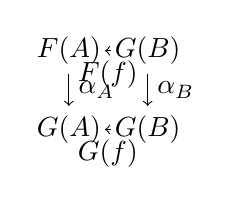
\begin{tikzpicture}[node distance=1cm,auto]
      \node (FA) {$F(A)$};
      \node (GA) [below of=FA] {$G(A)$};
      \node (FB) [right of=FA] {$G(B)$};
      \node (GB) [below of=FB] {$G(B)$};
      \draw[->] (FA) to node {$F(f)$} (FB);
      \draw[->] (GA) to node {$G(f)$} (GB);
      \draw[->] (FA) to node {$\alpha_A$} (GA);
      \draw[->] (FB) to node {$\alpha_B$} (GB);
    \end{tikzpicture}
    \fi

    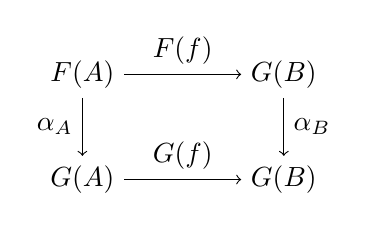
\begin{tikzpicture}
      \matrix (mat) [matrix of nodes, column sep=1.5cm, row sep=0.75cm]{
        \node (FA) {$F(A)$}; &
        \node (FB) {$G(B)$}; \\
        \node (GA) {$G(A)$}; &
        \node (GB) {$G(B)$}; \\
      };
      \draw[->] (FA) to node [above] {$F(f)$} (FB);
      \draw[->] (GA) to node [above] {$G(f)$} (GB);
      \draw[->] (FA) to node [left] {$\alpha_A$} (GA);
      \draw[->] (FB) to node [right] {$\alpha_B$} (GB);
    \end{tikzpicture}
  \end{center}
\end{defn}

\begin{bem}
  Ist $H : \mathcal{C} \to \mathcal{D}$ ein weiterer Funktor und $\beta : G \to H$ eine weitere natürliche Transformation, so ist $\beta \alpha : F \to H$ definiert durch
  \[ (\beta \alpha)_X \coloneqq \beta_X \circ \alpha_X : F(X) \to H(X) \]
  eine natürliche Transformation zwischen $F$ und $H$.
\end{bem}

\begin{bem}
  Für zwei Kategorien $\mathcal{C}$ und $\mathcal{D}$ gibt es die \emph{Funktorkategorie} $\left[\mathcal{C}, \mathcal{D}\right]$ der Funktoren zwischen $\mathcal{C}$ und $\mathcal{D}$ mit natürlichen Transformation als Morphismen.
\end{bem}

\begin{defn}
  Die Isomorphismen der Funktorkategorie $\left[\mathcal{C}, \mathcal{D}\right]$ heißen \emph{natürliche Isomorphismen}.
\end{defn}

\begin{lem}
  Eine natürliche Transformation $\eta : F \to G$ ist genau dann ein natürlicher Isomorphismus, wenn alle Komponenten $(\eta_X : F(X) \to G(X))_{X \in \Ob \mathcal{C}}$ Isomorphismen sind.
\end{lem}

\begin{bsp}
  Sei $** \coloneqq * \circ * : \mathbf{Vect}_k \to \mathbf{Vect}_k$ der Bidualisierungsfunktor. Es gibt eine nat. Transformation $\eta : \Id_{\mathbf{Vect}_k} \to **$ gegeben durch
  \[ \eta_V(v \in V) \coloneqq (\phi \mapsto \phi(v)). \]
  Für endlichdimensionale VR $V$ ist $\eta_V$ ein Isomorphismus, also ist $\eta|\mathbf{FinVect}_k : \Id_{\mathbf{FinVect}_k} \to **$ ein natürlicher Isomorphismus.
\end{bsp}

% Ausgelassen: Beispiel Kategorienäquivalenz: Kategorie der lokalkompakten Hausdorffräume ist äquivalent zur Kategorie der punktierten kompakten Hausdorffräume mittels des Einpunktkompaktifizierungs-Funktors

% Kapitel: Überlagerungen

\begin{defn}
  Seien $X, Y$ topologische Räume.
  \begin{itemize}
    \item Eine Teilmenge $Y \subset Y$ wird durch eine stetige Abbildung $p : X \to Y$ \emph{gleichmäßig überlagert}, falls es einen diskreten Raum $D$ und einen Homöomorphismus
    \[
      \phi : p^{-1}(U) \xrightarrow{\approx} U \times D
      \quad \text{mit} \quad
      p = \pi_1 \circ \phi
    \]
    gibt, wobei $\pi_1 : X \times D \to X$ die Projektion ist.
    % Ausgelassen: Kommutatives Diagramm
    \item Die Abbildung $p$ heißt \emph{Überlagerung}, falls jeder Punkt in $Y$ eine durch $p$ gleichmäßig überlagerte Umgebung besitzt.
  \end{itemize}
\end{defn}

\begin{bsp}
  $\R \to S^1, \enspace t \mapsto e^{2 \pi it}$ ist eine Überlagerung.
\end{bsp}

\begin{bem}
  Sei $p : X \to Y$ eine Überlagerung, $Y$ zshgd. Dann ist
  \[ Y \to \N_{\geq 1} \cup \{ \infty \}, \quad y \mapsto \text{\#} (p^{-1}(y)) \]
  konstant, da lokalkonstant.
  Falls $d = \text{\#} (p^{-1}(y))$ endlich ist, heißt $p$ eine \emph{$d$-blättrige} Überlagerung. Ansonsten heißt $p$ eine \emph{unendliche Überlagerung}. Eine Überlagerung mit mehr als einem Blatt heißt \emph{nichttriviale Überlagerung}.
\end{bem}

\begin{defn}
  Eine stetige Abbildung $p : X \to Y$ heißt \emph{lokaler Homöomorphismus}, falls für alle $x \in X$ eine offene Umgebung $U_x$ von $x$ existiert, sodass $p|_{U_x} : U_x \to p(U_x)$ ein Homöomorphismus ist.
\end{defn}

\begin{lem}
  Jede Überlagerung ist ein lokaler Homöomorphismus.
\end{lem}

\begin{prop}
  Sei $p : X \to Y$ eine Überlagerung, $\gamma : \I \to Y$ ein Weg und $x \in X$ mit $p(x) = \gamma(0)$. Dann gibt es einen eindeutig bestimmten Weg $\tilde{\gamma} : \I \to X$ mit $\tilde{\gamma}(0) = x$ und $p \circ \tilde{\gamma} = \gamma$.
\end{prop}

% Vorlesung vom 16.6.2014

\begin{satz}[Homotopie-Liftungsthm]
  Sei $p : X \to Y$ eine Überlagerung und $F : W \times \I \to Y$ eine Homotopie. Sei $\tilde{f} : W \to X$ eine Liftung von $F(\blank, 0)$, d.\,h. $p \circ \tilde{f} = F(\blank, 0)$. Dann existiert eine Homotopie $\widetilde{F} : W \times \I \to X$ mit $\widetilde{F}(\blank, 0) = \widetilde{f}$ und $p \circ \widetilde{F} = F$.
\end{satz}

\begin{kor}
  Seien $\gamma_0, \gamma_1$ Wege in $Y$ mit $\gamma_0 \simeq \gamma_1 \rel \{ 0, 1 \}$ und $\widetilde{\gamma_0}, \widetilde{\gamma_1} : \I \to X$ Liftungen von $\gamma_0$ und $\gamma_1$ mit dem gleichen Anfangspunkt $\widetilde{\gamma_0}(0) = \widetilde{\gamma_1}(0) = x_0 \in X$. Dann gilt $\widetilde{\gamma_0}(1) = \widetilde{\gamma_1}(1)$ und $\widetilde{\gamma_0} \simeq \widetilde{\gamma_1} \rel \{ 0, 1 \}$.
\end{kor}

\begin{kor}
  Sei $\gamma : \I \to Y$ ein geschl. Weg homotop zu einem konstanten Weg $\rel \{ 0, 1 \}$. Dann ist jeder Lift $\widetilde{\gamma} : \I \to X$ auch ein geschl. Weg und homotop zu einem konstanten Weg $\rel \{ 0, 1 \}$.
\end{kor}

\begin{kor}
  Sei $Y$ ein wegzshgder Raum, $p : X \to Y$ eine wegzshgde nichttriviale Überlagerung. Ist $y_0 \in Y$, so gilt $\pi_1(Y, y_0) \not= 1$.
\end{kor}

\begin{kor}
  $\R P^2 \not\approx S^2$, da die Quotientenabb. $S^2 \to S^2/{\sim} = \R P^2$ eine nichttriviale Überlagerung und $S^2$ einfach zshgd ist.
\end{kor}

\begin{prop}
  Die Abbildung $p : \R \to S^1, t \mapsto e^{2 \pi i t}$ ist eine Überlagerung von $S^1$. Bezeichne für geschl. Wege $f : \I \to S^1$ mit $f(0) = f(1) = 0$ mit $\tilde{f}$ die Liftung von $f$ mit $\tilde{f}(0) = 0$. Dann ist
  \[ \mathrm{deg} : \pi_1(S^1, 0) \to \Z, \quad [f] \mapsto \tilde{f}(1) \in \Z \]
  ein Gruppenisomorphismus.
\end{prop}

\begin{defn}
  Stetig Abbildungen $f : S^1 \to S^1$ mit $f(1) = 1$ können als geschlossene Wege $\I \to S^1$ aufgefasst werden. Dann heißt $\deg f \in \Z$ der \emph{Abbildungsgrad} von $f$.
\end{defn}

\begin{prop}
  $\deg(z \mapsto z^n : S^1 \to S^1) = n$ für alle $n \in \Z$.
\end{prop}

% Vorlesung vom 18.6.2014

% TODO: Abbildungsgrad für beliebige Abbildungen $S^1 \to S^1$

\begin{kor}[Fundamentalsatz der Algebra]
  Jedes nicht-konstantes Polynom mit komplexen Koeffizienten besitzt eine Nullstelle in $\C$.
\end{kor}

% Ausgelassen: Liftungsproblem

\begin{defn}
  Ein topol. Raum $X$ heißt \emph{lokal wegzusammenhängend}, falls für alle $x \in X$ und Umgebungen $U_x \subseteq X$ von $x$ eine wegzshgde Umgebung $V_x \subseteq U_x$ von $x$ existiert.
\end{defn}

\begin{satz}[Liftungstheorem]
  Sei $p : X \to Y$ eine Überlagerung, $W$ wegzshgd und lokal wegzshgd, $f : W \to Y$ stetig, $x_0 \in X$, $w_0 \in W$ mit $y_0 \coloneqq p(x_0) = f(w_0)$. Dann existiert eine stetige Abbildung $\tilde{f} : W \to X$ mit $p \circ \tilde{f} = f$ und $\tilde{f}(w_0) = x_0$ genau dann, wenn
  \[ f_*(\pi_1(W, w_0)) \subseteq \im (p_* : \pi_1(X, x_0) \to \pi_1(Y, y_0)). \]
  In diesem Fall ist die Liftung $\tilde{f}$ eindeutig.
\end{satz}

\begin{defn}
  Eine \emph{Decktransformation} einer Überlagerung $p : X \to Y$ ist ein Homöomorphismus $\phi : X \to X$ mit $p \circ \phi = p$. Ihre Menge bildet mit der Abbildungs-Komposition eine Gruppe $\Deck(p)$.
\end{defn}

\begin{kor}
  Seien $p : X \to Y$ eine Überlagerung, $x_0, x_1 \in X$ mit $p(x_0) = p(x_1)$. Ist $X$ einfach zshgd und lokal wegzshgd, so gibt es genau eine Decktransformation $\phi : X \to X$ mit $\phi(x_0) = x_1$.
\end{kor}

% Vorlesung vom 23.6.2014

\begin{defn}
  Eine Überlagerung $p : X \to Y$ heißt \emph{universell}, falls $p$ surjektiv, $X$ einfach zshgd und lokal wegzshgd ist.
\end{defn}

\begin{prop}
  Seien $p : X \to Y$ und $p' : X' \to Y$ universelle Überlagerungen. Dann gibt es einen Homöomorphismus $\phi : X \to X'$ mit $p' \circ \phi = p$.
\end{prop}

Für $p : (X, x_0) \to (Y, y_0)$ eine universelle Überlagerung und $g = [\gamma] \in \pi_1(Y, y_0)$ sei $\tilde{\gamma}$ der Lift von $\gamma$ mit $\gamma(0) = x_0$. Sei $\psi_g \in \Deck(p)$ die eindeutige Decktransformation mit $\psi_g(x_0) = \tilde{\gamma}(1)$.

\begin{prop}
  Die Abbildung $\Psi : \pi_1(Y, y_0) \to \Deck(p)$, $g \mapsto \psi_g$ ist ein Gruppenisomorphismus.
\end{prop}

% TODO: Hilfsdefinition: Transitive Gruppenwirkung

\begin{prop}
  Sei $p : X \to Y$ eine Überlagerung, $X$ wegzshgd und lokal wegzshgd und $G \subset \Deck(p)$ eine Untergruppe. Angenommen, für alle $y \in Y$ und $x_0, x_1 \in p^{-1}(y)$ existiert $g \in G$ mit $g(x_0) = x_1$. Dann gilt $G = \Deck(p)$.
\end{prop}

\begin{defn}
  Eine \emph{Wirkung} oder \emph{Operation} einer Gruppe $G$ auf einem Raum $X$ ist ein Gruppenhomomorphismus $\phi : G \to \Aut_{\mathbf{Top}}{X}$.
\end{defn}

\begin{nota}
  Statt $\phi(g)$ schreibt man auch $\phi_g$ oder $g$.
\end{nota}

\begin{defn}
  Der \emph{Orbitraum} der Gruppenwirkung von $G$ auf $X$ ist
  \[
    X / G \coloneqq X / {\sim}
    \quad \text{mit} \quad
    x \sim y \coloniff \ex{g \in G} g(x) = y.
  \]
\end{defn}

% Ausgelassen: Beispiel: $S^2 / (\Z/2) = \R P^2$

\begin{defn}
  Eine Gruppenwirkung $\phi : G \to \Aut(X)$ heißt \emph{eigentlich diskontinuierlich}, falls jeder Punkt $x \in X$ eine Umgebung $U$ besitzt, so dass gilt: $\fa{g \in G} \phi_g(U) \cap U \not= \emptyset \implies g = e$.
\end{defn}

\begin{prop}
  Sei $X$ zshgd, lokal wegzshgd, $G \to \Aut(X)$ eine eigentlich diskontinuierliche Wirkung. Dann ist $p : X \to X/G$ eine Überlagerung mit Decktransformationsgruppe $G$.
\end{prop}

\begin{satz}
  Sei $X$ einfach zshgd und lokal wegzshgd. Die Gruppe $G$ wirke eigentlich diskontinuierlich auf $X$. Dann gilt für jeden Basispunkt $y_0 \in Y \coloneqq X / G$: $\pi_1(Y, y_0) \cong G$.
\end{satz}

\begin{bspe}
  \begin{itemize}
    \item $\pi_1(S^1) = \pi_1(\R / \Z) \cong \Z$
    \item $\pi_1(S^1 \times S^1) = \pi_1(\R^2 / \Z^2) \cong \Z^2$
    \item $\pi_1(\R P^2) = \pi_1(S^2 / (\Z/2)) \cong \Z/2$
  \end{itemize}
\end{bspe}

\end{document}